\documentclass[referee]{aa} % for a referee version
%\documentclass[onecolumn]{aa} % for a paper on 1 column  
%\documentclass[longauth]{aa} % for the long lists of affiliations 
%\documentclass[letter]{aa} % for the letters 
%\documentclass[bibyear]{aa} % if the references are not structured 
%                              according to the author-year natbib style
%
%\documentclass{aa}  
\newcommand{\bea}{\begin{eqnarray}}
\newcommand{\eea}{\end{eqnarray}}
\newcommand{\ben}{\begin{enumerate}}
\newcommand{\een}{\end{enumerate}}
\newcommand{\bi}{\begin{itemize}}
\newcommand{\ei}{\end{itemize}}
\newcommand{\bmi}[1]{\begin{minipage}{#1 cm}}
\newcommand{\emi}{\end{minipage}}
\renewcommand{\[}{\begin{equation}}
\renewcommand{\]}{\end{equation}}

\renewcommand{\rm}{\mathrm}
\def\inv{^{-1}}
\def\({\left(}
\def\r){\right)}
\def\b#1{\bm{#1}}
\def\Dd{D_{\rm{d}}}
\def\Dds{D_{\rm{ds}}}
\def\Ds{D_{\rm{s}}}
\def\la{\left<}
\def\ra{\right>}
\def\gammao{\gamma^{\text{obs}}}
\def\gammaoh{\hat{\gamma}^{\text{obs}}}
\def\epsilonsij{\epsilon_{a_i}\epsilon_{b_j}^*}
\def\epsilonsii{\epsilon_{a_i}\epsilon_{b_i}^*}
\def\deltafuncij{\Delta(\b\theta_{a_i}-\b\theta_{b_j})}
\def\d{\rm{d}}
\def\bthp{\b \theta' + \b \theta}
\def\bth{\b \theta'}
\def\i{\rm{i}}

%\newcommand{\todo}{\emph}

\usepackage{bm}
\usepackage{verbatim}
%
\usepackage{graphicx}
%%%%%%%%%%%%%%%%%%%%%%%%%%%%%%%%%%%%%%%%
\usepackage{txfonts}
\usepackage{subcaption}

%%%%%%%%%%%%%%%%%%%%%%%%%%%%%%%%%%%%%%%%
%\usepackage[options]{hyperref}
% To add links in your PDF file, use the package "hyperref"
% with options according to your LaTeX or PDFLaTeX drivers.
%
\usepackage{todonotes}
%\renewcommand{\todo}{\emph}
\begin{document} 


   \title{The Effects of Varying Depth in Cosmic Shear Surveys}

%   \subtitle{}

   \author{Sven Heydenreich\inst{1}%\fnmsep\thanks{sven@astro.uni-bonn.de}
          \and Peter Schneider\inst{1} 
          \and Hendrik Hildebrandt\inst{2,1}
          \and Catherine Heymans\inst{3} 
          \and Marika Asgari\inst{3}
          \and Chieh-An Lin\inst{3,5,6}
          \and Benjamin Joachimi\inst{4}
          \and Tilman Tr\"{o}ster\inst{3}
          }
   \institute{Argelander-Institut f\"ur Astronomie, Auf dem H\"ugel 71, 53121 Bonn, Germany 
\and 
Astronomisches Institut, Ruhr-Universit\"at Bochum, Universit\"atsstr. 150, 44801 Bochum, Germany 
\and
Institute for Astronomy, University of Edinburgh, Royal Observatory, Blackford Hill, Edinburgh EH9 3HJ, UK
\and
Department of Physics and Astronomy, University College London, Gower Street, London WC1E 6BT, UK
\and
Service d'Astrophysique, CEA Saclay, Orme des Merisiers, B\^at 709, 91191 Gif-sur-Yvette, France
\and 
Fenglin Veteran Hospital, 2 Zhongzheng Rd. Sec. 1, Fenglin Township, Hualien 97544, Taiwan
\\ \email{sven@astro.uni-bonn.de, peter@astro.uni-bonn.de}
             }

   \date{Received XXX; accepted XXX}

  \abstract
% context (optional)
   {Cosmic shear proves to be a powerful tool to study the properties of the Universe. The discrepancy in the parameter $S_8 = \sigma_8\sqrt{\Omega_{\rm{m}}/0.3}$ between measurements in the local Universe and the Cosmic Microwave Background motivates further investigation of yet unaccounted systematic biases. 
% aims
   Ground-based surveys are subject to a variation in depth caused by varying atmospherical conditions; we investigate and quantify the resulting effects. In particular, we check whether they introduce a bias to the resulting cosmological parameters and if they can be responsible for the occurrence of B-modes.
% methods
   We construct a semi-analytic model to estimate the impact on the shear correlation functions and analyse the implications for cosmological parameters. Furthermore, we construct COSEBIs of the correlation functions to quantify the occurring B-modes.
% results
   For the Kilo-Degree Survey this effect introduces an error in $\xi_\pm$ of the order of a few percent on small scales. We find that the resulting bias in $\Omega_{\rm m}$ and $\sigma_8$ will be significant in next-generation cosmic shear surveys. The parameter $S_8$ is especially robust against this modification. We find that the dependency of this effect on the underlying cosmology is not negligible. We also report the occurrence of B-modes, although at a not yet significant level.
% conclusions (optional)
   We conclude that the effects of varying depth for ground-based surveys on cosmological parameters are not yet significant, but should be accounted for in next-generation experiments. Due to the cosmology dependency, further analyses require a fast, analytical model for this effect.}

   \keywords{gravitational lensing --
                weak lensing --
                cosmic shear
               }

   \maketitle

%
%-------------------------------------------------------------------
\section{Introduction}
The discovery of cosmic shear has provided us with a new and powerful cosmological tool to investigate the standard model of cosmology and to determine its parameters. Contrary to the analysis of the Cosmic Microwave Background (CMB) by \citet{2018arXiv180706209P}, cosmic shear is more sensitive to the properties of the local Universe and thus provides an excellent consistency check for the standard model. Current cosmic shear surveys are especially sensitive to the parameter $S_8=\sigma_8 \sqrt{\Omega_{\rm m}/0.3}$, where $\sigma_8$ denotes the normalization of the matter power spectrum and $\Omega_{\rm m}$ is the matter density.
It is interesting to note that all three current major cosmic shear results report a lower $S_8$ than inferred from the CMB analysis: While \citet{2018arXiv180706209P} determined a value of $S_8 = 0.830 \pm 0.013$, \citet{2018arXiv180909148H} report $S_8 = 0.800^{+0.029}_{-0.028}$ from analysis of the Subaru Hyper Suprime-Cam survey, \citet[][hereafter H18]{2018arXiv181206076H} obtained $0.737_{-0.036}^{+0.040}$ from KiDS+VIKING data and the Dark Energy Survey \citep[DES,][]{2018PhRvD..98d3528T} arrived at $S_8=0.782\pm 0.027$. Also, \citet{2013MNRAS.432.2433H} report $S_8 = 0.759 \pm 0.020$ from their analysis of CFHTLens data. Combined analyses of DES and KiDS data \citep{Joudaki:2019} yields even higher tension with the value determined for $S_8$ by the Planck Collaboration\todo{cite marikas new paper here as soon as it is there}. This discrepancy has received a lot of attention \citep{2017MNRAS.471.1259J,2016MNRAS.459..971K}. It could be interpreted as a statistical coincidence, a sign of new physics like massive neutrinos \citep{2014PhRvL.112e1303B}, time-varying dark energy or modified gravity \citep{2016A&A...594A..14P}; or as the manifestation of a systematic effect, either in the cosmic shear surveys or in the Planck mission \citep{2016ApJ...818..132A}, that is not yet accounted for. 

For current cosmic shear surveys, the estimated systematic error is of comparable size to the statistical error, implying that for next-generation surveys, a significant reduction of systematic errors is necessary \citep[][hereafter H17]{2017MNRAS.465.1454H}. With surveys like the Large Synoptic Survey Telescope \citep[LSST,][]{Ivezic:2008} and Euclid \citep{Laureijs:2011} soon to start, systematic effects in gravitational lensing have received a large amount of attention \citep{2018arXiv181002353A,2019arXiv190207439B,2019arXiv190109488S}. %\todo{Citations.. \citet{2017MNRAS.464.1676A} has a few...}

To check for remaining systematics, a weak lensing signal can be divided into two components, the so-called E- and B-modes \citep{2002ApJ...568...20C,2002A&A...389..729S}. To leading order, B-modes can not be created by astrophysical phenomena and are thus an excellent test for remaining systematics. The most useful E- and B-mode decomposition for cosmic shear surveys is provided by Complete Orthogonal Sets of E- and B-mode Integrals \citep[COSEBIs,][hereafter S10]{2010A&A...520A.116S}, as it can easily be applied to real data. Note that the non-existence of B-modes does not necessarily imply that the sample is free of remaining systematics.

One systematic effect is the variation of depth in a survey. While effects like Galactic extinction or dithering strategies do play a role in every survey, this work focuses on the effects caused by varying atmospheric conditions that are found in ground-based surveys. To first order, this variation can be modelled by a piece-wise constant depth function, which varies from pointing to pointing. In this work we assume the specifications of the Kilo-Degree Survey \citep[KiDS,][]{Kuijken:2015}, namely an assembly of $1\,\text{deg}^2$ square fields. 

The depth of a pointing primarily influences the number density as well as the average redshift of galaxies, meaning that a variation in depth is responsible for a correlation between those two quantities (see Fig. \ref{fig:nz_of_meanz}). \todo{I see why you would like to move this further down. However, I feel like this plot would make a nice Fig. 1, that captures the essence of what this paper is trying to analyse -- The effect of an artificial correlation between number density and redshift. I feel like the confusion caused by how exactly the plot is calculated is worth it to not have Fig. 2 (which is not that essential) as new Fig. 1. However, if you still feel like this figure would be better off further down, I will move it.}
%
\begin{figure}
\centering
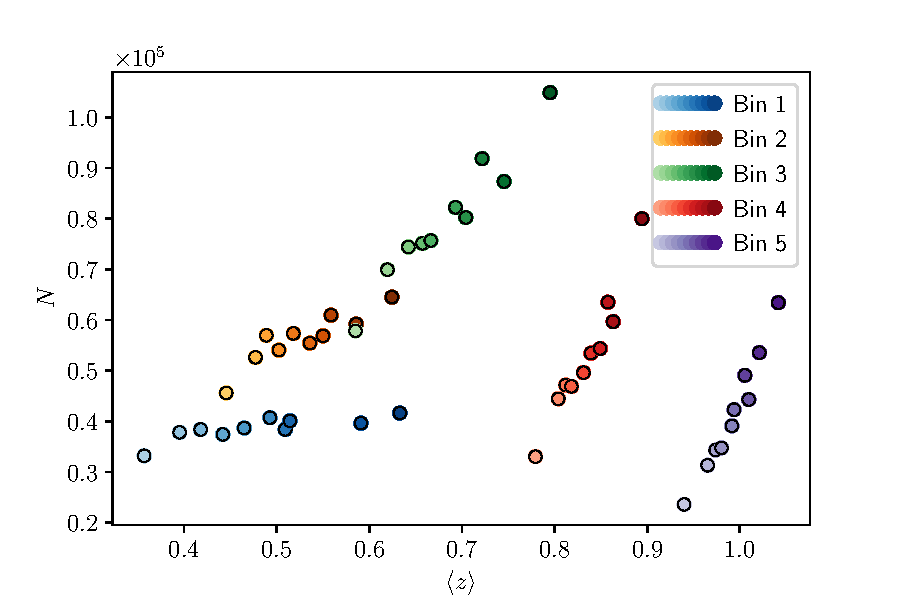
\includegraphics[width=0.7\linewidth]{images/cov_nz_meanz.pdf}
\caption{Galaxy number density $N$ and average redshift $\la z\ra$ in the KiDS+VIKING-450 (KV450) survey \citep{Wright:2018} survey in pointings of different depth for each of the five tomographic bins used in H18. Each colour corresponds to one redshift bin of H18, the fainter points denote pointings of shallower depth. Details on how the data were obtained are described in Sec. \ref{sec:xipm_semianalytic}.}
\label{fig:nz_of_meanz}
\end{figure}
%
In Sect. \ref{sec:modelling_single_lens} we will introduce a simple toy model to understand this effect and analyze the impact on the cosmic shear power spectrum. In Sect. \ref{sec:xipm} we will estimate the effect on the shear correlation functions $\xi_\pm$ using two different models. We will present our results in Sect. \ref{sec:results}. In Sect. \ref{sec:discussion} we will discuss our results and comment on the impacts of our used simplifications. We will assume the standard weak gravitational lensing formalism, a summary of which can be found in \citet{2001PhR...340..291B}.

%-------------------------------------------------------------------

\section{Modelling the power spectrum}
\label{sec:modelling_single_lens}
For our first analysis we assume that all the matter between sources and observer is concentrated in a single lens plane of distance $D_{\rm d}$ from the observer. If we now distribute sources at varying distances $D_{\rm s}$, then the convergence $\kappa$ varies according to $\kappa \propto D_{\rm{ds}}/D_{\rm s}$. 
% Following \citet{1993ApJ...404..441K}, we can simulate the shear $\gamma$ from the convergence by convolution with the kernel \[
%\mathcal{D}(\bm{\theta}) = \frac{\theta_2^2-\theta_1^2-2i\theta_1\theta_2}{\pi |\bm{\theta}|^4}\, .
%\]

%Similarly, an observer that measures the shear $\gamma$ can reconstruct the convergence $\kappa$ by convolution with the kernel $\mathcal{D}^*$, where ${}^*$ denotes the complex conjugate. Assuming that the optical depth, and thus the source redshift populations, vary between pointing, an observer will measure a shear-signal that is modified by a depth-function $W(\bm{\theta}) = 1-w(\bm{\theta})$, where $\langle w(\bm{\theta})\rangle=0$ holds. The reconstruction of the observed convergence $\kappa^{\rm obs}$ will thus not yield the original convergence. In particular there is no reason why the convolution with a complex kernel should have a nonzero imaginary part. This allows us to separate our received signal into E- and B-modes following \[
%	\kappa = \kappa^E+i\kappa^B\, ,
%\]
%where $B$-Modes can not be generated by a lensing signal and are thus a tracer of remaining systematics.
%2002A&A...389..729S SRC

Assuming that the depth, and thus the source redshift populations, varies between pointings of the camera, an observer will measure a shear-signal that is modified by a step-like depth-function $\gammao(\b\theta)=W(\b \theta)\gamma(\b\theta)$, where $W$ is proportional to the mean of the lensing efficiency $\Dds/\Ds$ of one pointing and $\gamma$ denotes the shear that this pointing would read if it were of average depth.
We can parametrize $W$ as $W(\bm{\theta}) = 1+w(\bm{\theta})$, where $\langle w(\bm{\theta})\rangle=0$ holds. 
In accordance to the definition of the shear power spectrum \begin{equation}
\la \hat{\gamma}(\b\ell)\,\hat{\gamma}^*(\b\ell')\ra = (2\pi)^2\delta(\b\ell-\b\ell')P(|\b\ell|) \, ,
\label{eq:original_power_spectrum}
\end{equation}
where $\hat{\gamma}$ denotes the Fourier transform of $\gamma$, we define the observed power spectrum via \begin{equation}
P^{\text{obs}}(\b\ell) \equiv \frac{1}{(2\pi)^2}\int \d^2 \ell'\,  \la \gammaoh(\b \ell)\, \gammaoh {}^*(\b \ell')\ra \, .
\end{equation}
Note that due to the depth-function both the assumptions of homogeneity and isotropy break down, which means that we can neither assume isotropy in the power spectrum, nor can we assume that $\la \gammaoh(\b \ell) \gammaoh {}^*(\b \ell')\ra$ vanishes for $\b\ell\neq\b\ell'$.
To model a constant depth on each individual pointing $\b \alpha$, we can choose random variables $w_{\b \alpha}$, that only need to satisfy $\langle w_{\b \alpha}\rangle=0$, and parametrize $w(\b\theta)$ as 
\begin{equation}
w(\b \theta) = \sum_{\b \alpha \in \mathbb{Z}^2} w_{\b \alpha} \Xi(\b \theta-L\b \alpha)\text{ , with the Box-Function } \Xi(\b \theta) = \begin{cases}
1 \qquad \b \theta\in \left[-\frac{L}{2},\frac{L}{2}\right]^2 \\
0 \qquad \text{else}
\end{cases},
\label{eq:defweightf}
\end{equation}
where $L$ is the length of one pointing.
Following the calculations in Appendix \ref{sec:calc of PS}, we derive 
\begin{equation}
P^{\text{obs}}(\b \ell)  =  P(\b \ell) + \la w^2\ra \int\frac{\text{d}^2\b k}{(2\pi)^2}\,\hat{\Xi}(\b \ell-\b k)\, P(\b k)\, ,
\end{equation}
where $\la w^2\ra \equiv \la w_{\b \alpha}^2\ra$ is the dispersion of the depth-function and $\hat{\Xi}$ is the Fourier transform of a box-function, which is a 2-dimensional sinc-function (compare \ref{sec:calc of PS}).
The observed power spectrum $P^{\text{obs}}$ is thus composed of the original power spectrum $P(\ell)$ from Eq. \eqref{eq:original_power_spectrum}, plus a convolution of the power spectrum with a sinc-function, scaling with the variance of the function $w(\b\theta)$. In particular, the power spectrum is not isotropic anymore.

%-------------------------------------------------------------------

\section{Modelling the shear correlation functions}
\label{sec:xipm}
Convenient measures to infer cosmological information from observational data are the shear correlation functions $\xi_\pm$, which are defined as \[
\xi_\pm(\theta) = \la \gamma_{\rm t}\gamma_{\rm t}\ra(\theta) \pm \la \gamma_\times\gamma_\times\ra(\theta) \, .
\]
Here, $\gamma_t$ and $\gamma_\times$ denote the tangential- and cross-component of the shear for a galaxy pair with respect to their relative orientation \citep[see][]{2002A&A...396....1S}.
The shear correlation functions are the prime estimators to quantify a cosmic-shear signal, since it is simple to include a weighting of the shear measurements into the correlation functions and, contrary to the power spectrum, one does not have to worry about the shape of the survey footprint or masked regions, or model the noise contribution. 
\subsection{Using an analytic model}
\label{sec:xipm_analytic}
For a first simple analysis we will assume that a deeper redshift distribution just yields a stronger shear signal, in the sense that the shear field for a deeper redshift distribution gets multiplied by a weight $W>1$. This is equivalent to the assumption that all matter between source and observer is concentrated in a single lens plane from the previous Section. While this is not true for a 3-dimensional lensing matter distribution, it should be a reasonable first approximation for small variations in mean source redshift. Additionally, we assume that a higher depth does not only lead to a stronger average shear, but also to a higher galaxy number density, implying a correlation between those two quantities.

Let $N^i(\b \theta),N^j(\b\theta)$ be the average weighted number of galaxies per pointing in redshift bins $i$ and $j$ and let $W^i(\b \theta),W^j(\b\theta)$ be the weighting of average shear. The observed correlation functions $\xi^{ij,\text{obs}}_\pm(\theta)$ now change from one of uniform depth, $\xi_\pm^{ij,\rm{uni}}(\theta)$, via \citep[see][]{2002A&A...396....1S}
\begin{align}
\xi^{ij,\text{obs}}_\pm(\theta) = & \frac{\la N^i(\bth)N^j(\bthp)\gamma^{i,\rm{obs}}_{\rm t}(\bth)\gamma^{j,\rm{obs}}_{\rm t}(\bthp)\ra }{\la N^i(\bth)N^j(\bthp)\ra} \pm \frac{\la N^i(\bth)N^j(\bthp)\gamma^{i,\rm{obs}}_\times(\bth)\gamma^{j,\rm{obs}}_\times(\bthp)\ra }{\la N^i(\bth)N^j(\bthp)\ra} \nonumber\\
 = & \frac{\la N^i(\bth)N^j(\bthp)W^i(\bth)W^j(\bthp)\ra}{\la N^i(\bth)N^j(\bthp)\ra} \xi_{\pm}^{ij,\rm{uni}}(\theta) \, ,
 \label{eq:xipmblub1}
 \end{align}
 where the average $\la\ldots\ra$ represents both an ensemble average as well as an average over the position $\bth$.
 Assuming that depth of different pointings is uncorrelated implies that the same holds for the functions $W$ and $N$. This means that the only important property of a galaxy pair is whether or not they lie in the same pointing. We want to denote the probability that a random galaxy pair of separation $\theta$ lies in the same pointing, by $E(\theta)$. This function is depicted in Fig. \ref{fig:eoftheta_lin}, and an analytical expression is derived in App. \ref{sec:model_e}.
 
\begin{figure}
 \centering
 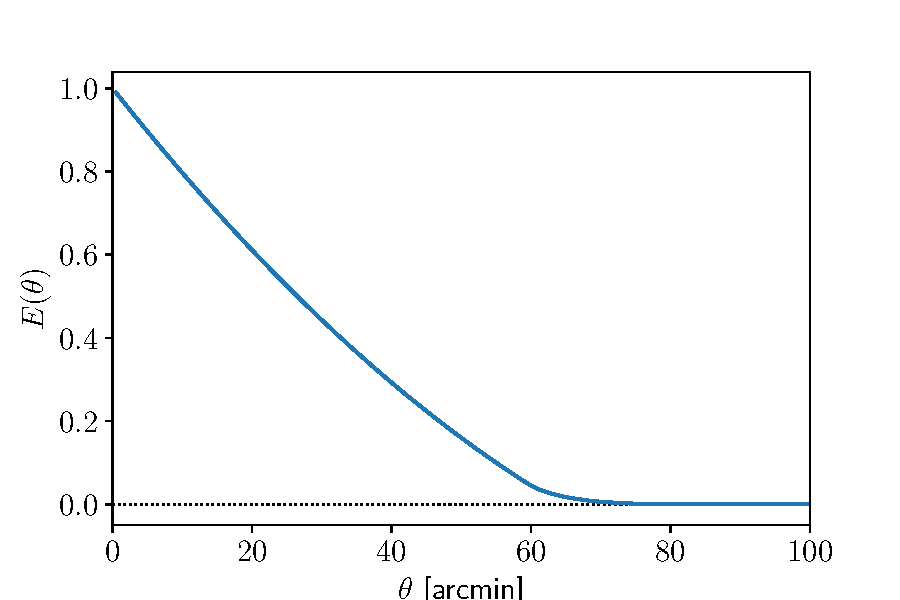
\includegraphics[width=0.5\textwidth]{images/eoftheta.pdf}
 \caption{Probability $E(\theta)$ that a random pair of galaxies of distance $\theta$ lie in the same $1\deg ^2$ pointing.}
 \label{fig:eoftheta_lin}
\end{figure}

To compute the modified shear correlation functions, we parametrize the number densities \linebreak$N^{i}(\b \theta)=\la N^{i} \ra [1+n^{i}(\b \theta)]$ and the weight $W^{i}(\b \theta)=1+w^{i}(\b \theta)$ and, as in Eq. \eqref{eq:defweightf}, interpret $n^{i}(\b \theta)$ as a function with average $\la n^{i} \ra = 0$ that is constant on each pointing. We can see that $\la n^i(\bth)n^j(\bthp)\ra = E(\theta)\la n^i(\bth)n^j(\bth)\ra = E(\theta)\la n^i n^j \ra$ holds and compute:
\begin{align}
&\frac{\la N^i(\bth)N^j(\bthp)W^i(\bth)W^j(\bthp)\ra}{\la N^i\ra \la N^j\ra } \nonumber\\
&\qquad =  1 + \la n^iw^i\ra + \la n^j w^j\ra + E(\theta)\left[ \la n^in^j\ra + \la n^i w^j \ra  + \la n^jw^i\ra + \la w^iw^j\ra + \la n^in^jw^i\ra + \la n^in^jw^j\ra + \la n^iw^iw^j\ra \right. \nonumber\\
&\qquad\quad \left. + \la n^jw^iw^j\ra + \la n^in^jw^iw^j\ra  \right] \, .
 \end{align}
Ignoring correlations higher than second order in $n^i$ and $w^i$,\footnote{It is not inherently obvious that this is a valid assumption. However, after performing calculations with and without higher order correlations, the highest difference between the outcomes of both equations was less then $5\times 10^{-4}$.} and performing the same calculation for the denominator of Eq.\,\eqref{eq:xipmblub1}, we get
 \begin{align}
 \xi^{ij,\rm{obs}}_\pm(\theta) = \frac{1 + \la n^iw^i\ra + \la n^jw^j\ra + E(\theta)\left[\la n^in^j\ra + \la n^iw^j\ra + \la n^j w^i\ra + \la w^iw^j\ra\right]}{1+E(\theta)\la n^i n^j\ra }\xi^{ij,\rm{uni}}_\pm (\theta) \, .
 \end{align}
 A model correlation function for a cosmic shear survey is usually calculated by taking the average redshift distribution of a redshift bin, weighted by the number density.
 Ignoring that the depth is correlated on scales of one pointing (here at $\theta \leq \sqrt{2}^\circ$) is equivalent to setting $E(\theta)\equiv 0$. Note that there is still a correlation between $N$ and $W$ for the same galaxy.
%For the calculation of the reference correlation functions $\xi_\pm^{ij}(\theta)$ we distribute the \textit{same} galaxies into our survey, only this time we will not order their weightings $W$ or their number densities $N$ by pointing. We can imagine this by cutting the footprint into infinitesimal elements $\d^2\b\theta$, and redistributing those at random. When we calculate the correlation function of this survey, we note that $\la n^i(\bth)\ra \la n^j(\bthp)\ra = 0$ holds for $\b\theta\neq \b 0$, as the two corresponding infinitesimal elements have uncorrelated weighting and number density. This is equivalent to setting $E(\theta)\equiv 0$.
 Performing the same calculations as above, this yields a relation between the correlation function of uniform depth $\xi_\pm^{ij,\rm{uni}}$ and the one that is usually modelled, $\xi_\pm^{ij}$:
\begin{equation}
\xi_\pm^{ij}(\theta) = \left(1+\la n^iw^i\ra + \la n^jw^j\ra \right)\xi_\pm^{ij,\rm{uni}}(\theta)\, .
\end{equation}
When an observer now calculates the model correlation functions $\xi^{ij}_\pm$ without accounting for varying depth between pointings, the ratio between modelled and observed correlation functions becomes: \begin{equation}
\frac{\xi^{ij}_\pm(\theta)}{\xi_\pm^{ij,\rm{obs}}(\theta)} \approx \frac{1+\la n^iw^i\ra+\la n^jw^j\ra + E(\theta)\la n^in^j\ra}{1 + \la n^iw^i\ra + \la n^jw^j\ra + E(\theta)\left[\la n^in^j\ra + \la n^iw^j\ra + \la n^j w^i\ra + \la w^iw^j\ra\right]}
\, .
\end{equation}
It is interesting to note that $\xi^{ij}_\pm = \xi_\pm^{ij,\rm{obs}}$ holds wherever $E(\theta)=0$, so we expect the observed and the modelled correlation functions to be equivalent on scales where the depth is uncorrelated. 


%-------------------------------------------------

\subsection{Using a semi-analytic Model}
\label{sec:xipm_semianalytic}
The previously derived analytic model describes how varying depth between pointings modifies the correlation function due to the correlation between number density and average redshift of source galaxies. While this model serves as an intuitive first approximation, it completely ignores any effects from the large scale structure (LSS) between the closest and the most distant galaxy. Therefore, we do not expect this model to yield reliable, quantitative results for cosmic shear surveys.

Below we derive a more sophisticated model that includes the effects of the LSS. While it is computationally more expensive, it yields accurate results for cosmic shear surveys, which are sensitive to the exact redshift distributions of sources as well as the underlying cosmology.

An inspection of KiDS-data showed that the redshift distribution of sources is highly correlated with the depth in the $r$-band\todo{This is basically from unpublished data of a KV450 WG telecon. Should/can I cite something here?}. We thus chose to separate the survey into 10 percentiles, sorted by $r$-band depth, i.e. if a pointing had a shallower depth than 90\% of the other pointings, it would belong to the first percentile, and so on. For each percentile $m$ and each tomographic redshift bin $i$ we can extract a weighted number of galaxies $N^i_m$ and, a source redshift distribution $p^i_m(z)$ following the DIR method of H17\footnote{Instead of using the actual number of galaxies, we take the sum of their lensing weights, following H17. Due to this we account for different weighting of galaxies in the shear correlation functions as well as in the average redshift distribution.}. Asserting an arbitrary cosmological model, we can transform the source redshift distributions $p^i_m(z)$ into comoving distance probability distributions $\mathcal{L}^i_m(\chi)$.

Given two comoving distance probability distributions of sources $\mathcal{L}^i_m(\chi),\mathcal{L}^j_n(\chi)$, we can compute the shear correlation functions from the underlying matter power spectrum $P(\ell,\chi)$ via \citep[compare][]{1992ApJ...388..272K} \begin{align}
\label{eq:xipm-pkappa}
\xi_{\pm,mn}^{ij}(\theta) =& \int_0^\infty \frac{{\rm d}\ell\,\ell}{2\pi}\, J_{0,4}(\ell\theta)\, P^{ij}_{\kappa,mn}(\ell)\, , \\
\label{eq:pkappa-pdelta/lenseff}
P^{ij}_{\kappa,mn}(\ell) =& \frac{9 H_0^4\Omega_{\rm m}^2}{4c^4}\int_0^{\chi_{\rm{H}}} {\rm d}\chi\, \frac{g^i_m(\chi)g^j_n(\chi)}{a^2(\chi)}\, P_\delta\left(\frac{\ell}{f_K(\chi)},\chi\right)\, , \\
\label{eq:lenseff}
g^i_m(\chi) =& \int_\chi^{\chi_{\rm{H}}} {\rm d}\chi' \, \mathcal{L}^i_m(\chi') \, \frac{f_K(\chi'-\chi)}{f_K(\chi')}\, .
\end{align}
Here, $J_{0,4}$ denote the 0-th and 4-th order Bessel Functions, $f_K(\chi)$ is the comoving angular diameter distance and $\chi_{\rm{H}}$ is chosen such that $p_i(\chi)=0$ holds for all $\chi>\chi_{\rm{H}}$.

Using \eqref{eq:xipm-pkappa}, we can compute the model correlation functions $\xi_{\pm,mn}^{ij}(\theta)$ for each pair of percentiles $m,n$ and redshift bins $i,j$.\footnote{For the calculation of the shear correlation functions we use the \textsc{Nicaea}-program \citep{10.1093/mnras/stx2082}. Among other quantities, it calculates the shear correlation functions for a given cosmology and source redshift distribution. For the power spectrum on nonlinear scales, we use the method of \citet{2012ApJ...761..152T}.} When measuring the shear correlation functions of a survey, we take the weighted average of tangential and cross shears of all pairs of galaxies (compare H17). If, for a single pair of galaxies, one galaxy lies in the $m$-th percentile of redshift bin $i$ and the second one lies in the $n$-th percentile of redshift bin $j$, then their contribution to the observed correlation functions is, on average, $\xi_{\pm,mn}^{ij}(\theta)$. This means that if we know each of those single correlation functions, we can reconstruct the total correlation functions via a weighted average of the single functions. Formally, we define \[
\xi_\pm^{ij,\rm{obs}}(\theta) = \frac{\sum_{m,n} \mathcal{P}_{mn}^{ij}(\theta)\,\xi_{\pm,mn}^{ij}(\theta)}{\sum_{m,n} \mathcal{P}_{mn}^{ij}(\theta)}\, ,
\label{eq:def_xiobs}
\]
where $\mathcal{P}_{mn}^{ij}$ is a weighting of the correlation functions, which has to be proportional to the probability that a galaxy pair of separation $\theta$ comes from percentiles $m$ and $n$\todo{We \textit{could} completely scratch this derivation and just point to the Appendix; I personally feel that this approach is more intuitive than the more mathematical one of the appendix, but if the paper gets too long we definitely do not need two methods to derive the same equation.}. In this analysis, we will assume an infinitely large survey footprint with an uncorrelated distribution of depth. We will later discuss the validity of these assumptions as well as possible mitigation strategies. 

To calculate $\mathcal{P}_{mn}^{ij}(\theta)$ we imagine two arbitrary (infinitesimally small) surface elements $\d^2\b\theta_1,\d^2\b\theta_2$ of separation $\theta$ on the sky. For the case $m\neq n$ we know that a pair of galaxies contributing to $\mathcal{P}_{mn}^{ij}(\theta)$ has to lie in different pointings, else they would automatically be of the same percentile. The probability that the imagined surface elements are within different pointings is $[1-E(\theta)]$. Furthermore, the first element $\d^2\b\theta_1$ has to lie in percentile $m$, the probability of which is $1/10$. The pointing of the second element $\d^2\b\theta_2$ has to be of percentile $n$; the probability of that is also equal to $1/10$. The probability that a galaxy pair populates those surface elements is proportional to the weighted number of galaxies $N_m^i,N_n^j$. We get for $n\neq m$: \[
\mathcal{P}_{mn}^{ij}(\theta) = [1-E(\theta)]\frac{1}{100} N_m^i N_n^j\, .
\label{eq:pmnij_corr1}
\]
For the calculation of $\mathcal{P}_{mm}^{ij}(\theta)$ we have to account for a different possibility: In case that the galaxy lies in the same pointing [accounted for by the factor $E(\theta)$], it automatically is of the same percentile. We therefore set \[
\mathcal{P}_{mm}^{ij}(\theta) = E(\theta)\frac{1}{10} N_m^iN_m^j + [1-E(\theta)]\frac{1}{100} N_m^i N_m^j \, .
\label{eq:pmnij_corr2}
\]
We can then write $\mathcal{P}_{mn}^{ij}(\theta)$ as: \[
\mathcal{P}_{mn}^{ij}(\theta) = E(\theta)\frac{1}{10} N_m^iN_m^j\,\delta_{mn} + [1-E(\theta)]\frac{1}{100} N_m^i N_n^j \, ,
\label{eq:pmnij_uncorr}
\]
where $\delta_{mn}$ denotes the Kronecker delta.
Inserting this into Eq.\,\eqref{eq:def_xiobs}, we compute
\begin{align}
\xi_{\pm,mn}^{ij,\rm{obs}}(\theta) = & \frac{1}{C}\sum_{m=1}^{10} N_m^i \left\{ E(\theta) N_m^j \xi_{\pm,mm}^{ij}(\theta) + \frac{\big[1-E(\theta)\big]}{10}\sum_{n=1}^{10}N_n^j \xi_{\pm,mn}^{ij}(\theta)\right\}\, ,
\label{eq:correctionfunction1}
\end{align}
with the normalization
\[
C = \sum_{m=1}^{10} N_m^i \bigg[ E(\theta)  N_m^j + \frac{\big[1-E(\theta)\big]}{10}\sum_{n=1}^{10} N_n^j\bigg]\, .
\]
A mathematically more rigorous derivation of this function can be found in Appendix \ref{sec:calc of xipm}.

If we want to compute this for all 5 redshift bins of the KV450-survey, this forces us to calculate and coadd 1275 correlation functions\footnote{For each of the 15 pairs redshift bins we need to calculate 100 correlation functions, except for the pairs of bins with the same redshift, where only 55 correlation functions need to be calculated due to symmetry.}. Since we are investigating an effect that is of the order of a percent, even small numerical errors can add up, skewing the calculations. Additionally, calculating $10^3$ correlation functions is computationally expensive. However, if we examine Eq.~\eqref{eq:lenseff}, we see that the comoving distance distribution of sources enters linearly. This in turn implies that in Eqs.~\eqref{eq:pkappa-pdelta/lenseff} and \eqref{eq:xipm-pkappa}, both source distance distributions enter linearly, meaning that, instead of adding correlation functions, we can add their respective redshift distributions and compute the correlation functions of that. In particular, we can define the \textit{combined number of galaxies} $N^i$ and \textit{average comoving distance probability distribution} $\mathcal{L}^i(\chi)$ of tomographic bin $i$ as \[
N^i\equiv\sum_m N_m^i\, , \qquad \mathcal{L}^i(\chi) = \frac{\sum_m N_m^i \mathcal{L}_m^i(\chi)}{\sum_m N_m^i} \, .
\]
If we define $\xi^{ij}_\pm$ as the correlation functions between the average comoving distance distributions $\mathcal{L}^i(\chi)$ and $\mathcal{L}^j(\chi)$, we find: \begin{align}
\sum_{m,n}N_m^iN_n^j\xi^{ij}_{\pm,mn} = & \, \frac{9 H_0^4\Omega_{\rm m}^2}{4c^4} \sum_{m,n} N_m^i N_n^j \int_0^\infty \frac{{\rm d}\ell\,\ell}{2\pi}\, J_{0,4}(\ell\theta) \int_0^{\chi_{\rm{H}}} \frac{{\rm d}\chi}{a^2(\chi)}\, P_\delta\left(\frac{\ell}{f_K(\chi)},\chi\right) \\
& \int_\chi^{\chi_{\rm{H}}} {\rm d}\chi' \, \mathcal{L}^i_m(\chi') \, \frac{f_K(\chi'-\chi)}{f_K(\chi')}
\int_\chi^{\chi_{\rm{H}}} {\rm d}\chi'' \, \mathcal{L}^j_n(\chi'') \, \frac{f_K(\chi''-\chi)}{f_K(\chi'')} \\
 = & \,N^i N^j \, \frac{9 H_0^4\Omega_{\rm m}^2}{4c^4} \int_0^\infty \frac{{\rm d}\ell\,\ell}{2\pi}\, J_{0,4}(\ell\theta) \int_0^{\chi_{\rm{H}}} \frac{{\rm d}\chi}{a^2(\chi)}\, P_\delta\left(\frac{\ell}{f_K(\chi)},\chi\right) \\
& \int_\chi^{\chi_{\rm{H}}} {\rm d}\chi' \, \frac{\sum_m N_m^i \mathcal{L}^i_m(\chi')}{N^i} \, \frac{f_K(\chi'-\chi)}{f_K(\chi')}
\int_\chi^{\chi_{\rm{H}}} {\rm d}\chi'' \, \frac{\sum_n N_n^j \mathcal{L}^j_n(\chi'')}{N^j}  \, \frac{f_K(\chi''-\chi)}{f_K(\chi'')} \\
 = & \, N^iN^j\xi^{ij}_\pm\, .
\end{align}
Consequently, we can apply this to \eqref{eq:correctionfunction1}, yielding
\begin{equation}
\xi_{\pm}^{ij,\rm{obs}}(\theta) = \frac{1}{C}\left\{ E(\theta)\left[\sum_{m=1}^{10} N_m^iN_m^j \xi_{\pm,mm}^{ij}(\theta)\right] +\frac{\big[1-E(\theta)\big]}{10}\xi_\pm^{ij}(\theta)N^iN^j\right\}\, .
\label{eq:correctionfunction2}
\end{equation}
For each pair of redshift bins we thus only have to compute eleven correlation functions, which reduces the number of functions to compute from 1275 to 165.

%-------------------------------------------------------------------

\section{Results}
\label{sec:results}
Here we apply both the analytic and the semi-analytic method to model the data from the KiDS+VIKING-450 survey \citep[KV450,][]{Wright:2018}. While the application of the semi-analytic method is straightforward, for the analytic method we need to decide how to estimate the weight function $W$ from given redshift data. Following the separation of a survey into percentiles as in Sect. \ref{sec:xipm_semianalytic}, we define $W(\b\theta)\equiv W_n$ whenever $\b\theta$ is in a pointing of percentile $n$. For the determination of $W_n$ we tried two approaches:
 As a first method, following \citet{2006APh....26...91V,1997A&A...322....1B}, we estimate 
\[
W_n \propto \la z_n \ra ^{0.85}\, ,
\]
where $\la z_n\ra$ is the average redshift of percentile $n$. As a second method we define \[
W_n \propto \sqrt{ \la\gamma_{\rm{t}}\gamma_{\rm{t}}\ra (\theta_{\rm{ref}}) + \la \gamma_\times\gamma_\times\ra (\theta_{\rm{ref}})} = \sqrt{\xi_{+,nn}^{ij}(\theta_{\rm{ref}})}\, ,
\]
where the $\xi_{+,nn}^{ij}(\theta_{\rm{ref}})$ denotes the model correlation function defined in Sect. \ref{sec:xipm_semianalytic}, evaluated at a characteristic scale $\theta_{\rm{ref}}$, that needs to be chosen.

While the first method suffers from the fact that the power-law index only holds for sources of redshifts $1\lesssim z \lesssim 2$, the second method is sensitive to the angular range $\theta_{\rm{ref}}$, at which the shear correlation functions are evaluated, which is fairly arbitrary.

We applied both analytic methods and the semianalytic one to data from KV450, following the separation into tomographic bins as in H18, and computed the ratio between our model for the observed correlation function $\xi_{\pm}^{\rm{obs}}$, and the model correlation function ignoring variations in depth, $\xi_{\pm}$. 

We compare our models to the results measured from numerical simulations. Using a modified version (Joachimi, Lin, et al. in prep.) of Full-sky Lognormal Astro-fields Simulation Kit \citep[FLASK,][]{Xavier:2016}, we generated galaxy mocks with coherent clustering and lensing signals from lognormal fields. For each lognormal field, one mock with uniform depth and another one with variable depth were generated. In the variable case, we measured the depth of tiles in the KiDS-1000 data \citep{Kuijken:2019} and performed an analogous separation into 10 bins. Each depth bin can then be associated with a tomographic redshift set and the galaxy redshifts were sampled accordingly from one of the 10 distributions. We observed that the relation between depth and effective number density, as well as the one between depth and shape noise, is linear, so we sampled both quantities for each bin from a linear fit. In the uniform case, redshifts, number densities and shape noise were sampled from the average of these 10 tomographic sets. Finally, we compute the ratio of the average lensing signals from the two mocks. The number of realizations is 2000. Shape noise is omitted. The results can be seen in Fig.~\ref{fig:all_xis}.
	\begin{figure}
	\centering
	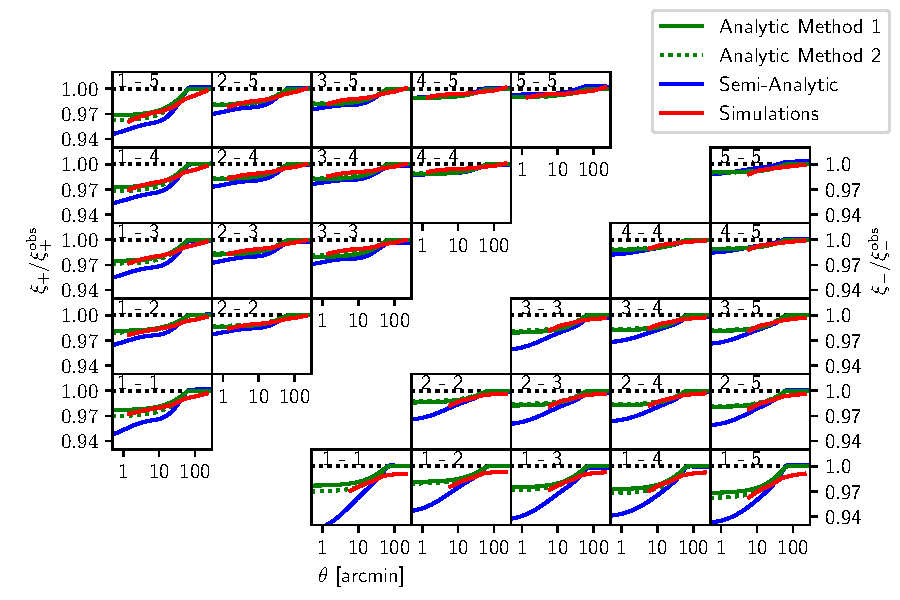
\includegraphics[width=1\textwidth]{images/xis_all1.pdf}
	\caption{The ratio of observed to modelled correlation functions for the analytic methods (green), the semi-analytic method (blue) and the numerical simulations (red) for a cross-correlation of all redshift bins. The numbers in the upper left corners correspond to the respective redshift bins, the upper left triangle depicts the ratios of $\xi_+$, whereas the lower right triangle depicts the ratios of $\xi_-$. For the characteristic scale $\theta_{\rm{ref}}$ of the second analytic method we chose $\theta_{\rm{ref}} \approx 11'$.}
	\label{fig:all_xis}
	\end{figure}
%We can see that for high redshift bins, the analytic and the semi-analytic methods are consistent, whereas for low redshift bins they significantly diverge. We explain this due to the facts that the analyic method uses simplifications that are redshift-dependent and only hold for small variations in redshift, which is not fulfilled in the low redshift bins.
We observe that for high-redshift bins, both analytic methods as well as the semi-analytic one yield consistent results. Due to the redshift-dependent index in the power law of the first analytic method, it is not able to accurately describe the effect for low redshift bins. The second analytic method, however, traces the semi-analytic one pretty well for $\xi_+$. As $\xi_-$ is affected much stronger by this effect, the analytic method is not able to trace this change.\footnote{The effect on $\xi_-$ is much stronger due to the fact that in Equation \eqref{eq:xipm-pkappa}, $\xi_+$ is computed by filtering the power spectrum with the 0-th order Bessel function. This function peaks at $\ell\theta=0$, meaning that for all values of $\theta$, the correlation function $\xi_+$ is sensitive to small values of $\ell$, corresponding to large separations $\theta$. However, $\xi_-$ is obtained by filtering with the 4-th order Bessel function, which peaks at approximately $\ell\theta\approx 5$, so for different $\theta$ this function is sensitive to varying parts of the convergence power spectrum. A more detailed analysis of this can be found in the Appendix of \citet{2017MNRAS.471.4412K}.}

The simulations and the models seem to be in rough agreement, but there are some differences. It is noticeable that in the simulations, the value $\xi_\pm/\xi_\pm^{\rm{obs}}$ consistently stays below unity, which can be attributed to the fact that the depth of different pointings is not completely uncorrelated, as was assumed in the models. Furthermore, we notice some strong features in the simulations at lower values of $\theta$.  As the noise of the simulated correlation functions increases for decreasing $\theta$,\footnote{The logarithmic bins for the correlation functions were chosen in H17 such that the signal-to-noise ratio is roughly equal for each bin. However, in the simulations we ignore shape-noise, such that our only noise contribution is sample variance, which increases at lower $\theta$.} and we take the ratio of two functions that are subject to noise, these features can be attributed to sample variance. In general, the semi-analytic model seems to over-estimate the effect compared to the simulations, which take the full distribution of depth into account. This slight discrepancy could be attributed to the fact that the simulations make use of the whole KiDS-1000 data, whereas the models rely on distributions extracted from KV450 data. % Additionlly, the simulations take the full variations in depth into account, which include both scales smaller than one pointing (especially dithering strategies) and scales larger than one pointing.

An additional difference between the models and simulations is that in the models we assume an infinite footprint, whereas the simulations were performed with the actual KiDS-1000 footprint. In Appendix \ref{sec:expand_eoftheta} we develop a model to extract the correction $\xi_\pm^{ij}/\xi_{\pm}^{ij,\rm{obs}}$ for a specific survey footprint. With this model we can estimate the impacts of a correlated distribution of depth, the sample variance of the depth-distribution and boundary effects. We find that for a quadratic footprint of $450\,\rm{deg}^2$ or $1000\,\rm{deg}^2$ with an uncorrelated depth-distribution, finite field effects are negligible.

As the next step we chose a fiducial cosmology $\b \Phi$ and computed reference correlation functions $\xi_\pm^{ij}(\theta,\b\Phi)$ for each pair of redshift bins $i,j$. Using our semi-analytic model in Sect.~\ref{sec:xipm_semianalytic}, we derived the observed correlation function $\xi_\pm^{ij,\rm{obs}}(\theta,\b\Phi)$ from those. Then we ran a Markov-Chain Monte Carlo simulation to check for the resulting bias in the inferred cosmological parameters, using the covariance-matrix computed in H18. As our main interest lies in the $\Omega_{\rm m}$ - $\sigma_8$ combination, we restricted our analysis to those two parameters. As can be seen in Fig.~\ref{fig:mcmc_kids}, the impact of varying depth is insignificant compared to the uncertainties. To get a rough estimate for the impact on future surveys, we divided our covariance-matrix by a factor of 30, to approximately account for the increased survey area of LSST and Euclid with respect to KV450. As can be seen in Fig.~\ref{fig:mcmc_euclid}, here the impact on both $\Omega_{\rm m}$ and $\sigma_8$ is significant. Conveniently it seems that the parameter $S_8$ is considerably more robust against this effect.

\begin{figure}
\begin{subfigure}{0.5\textwidth}
	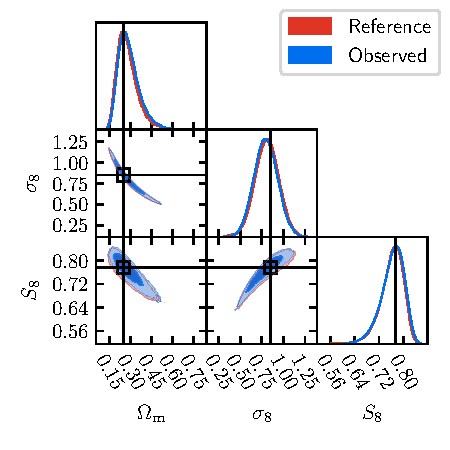
\includegraphics[width=\textwidth]{images/mcmc_kids.pdf}
	\caption{Bias for a KiDS-like Survey.}
	\label{fig:mcmc_kids}
\end{subfigure}
\begin{subfigure}{0.5\textwidth}
	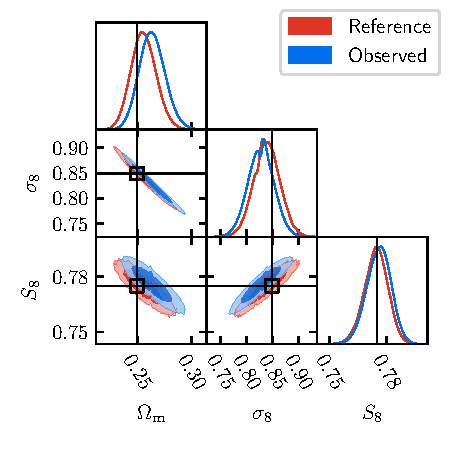
\includegraphics[width=\textwidth]{images/mcmc_euclid.pdf}
	\caption{Bias for a 'Euclid-like' Survey.}
	\label{fig:mcmc_euclid}
\end{subfigure}
\caption{Estimation of the bias caused by a variation of depth in a cosmic shear survey. Both simulations were computed using a fiducial cosmology of $\Omega_{\rm{m}}=0.25$ and $\sigma_8 = 0.85$.}
\end{figure} 

Calculating the correction $\xi_\pm^{ij}/\xi_\pm^{ij,\rm{obs}}$ for varying values of $\Omega_{\rm{m}}$ and $\sigma_8$ reveals a nontrivial dependence on the cosmology, which can be seen in Figure \ref{fig:comparecosmo}.

To estimate the B-modes created by this effect, we have extracted the \emph{Complete Orthogonal Sets of E- and B-Mode Integrals} (COSEBIS, compare S10), once of a reference set of correlation functions, to estimate numerical inaccuracies,\footnote{For a reference correlation function the B-Modes should be consistent with zero.} and then for the correlation functions that have been modified to account for a varying depth. We report a consistent B-mode behaviour across all redshift-bins, which can be seen in Figure \ref{fig:bmodes_cosebi}. It should be noted that the difference in E-modes is as large as the B-modes, which suggests that any significant change in the cosmological parameters due to a varying depth will also yield the significant detection of B-modes.\todo{add reference in the figure as soon as marika's paper is on arxiv}


\begin{figure}
\centering
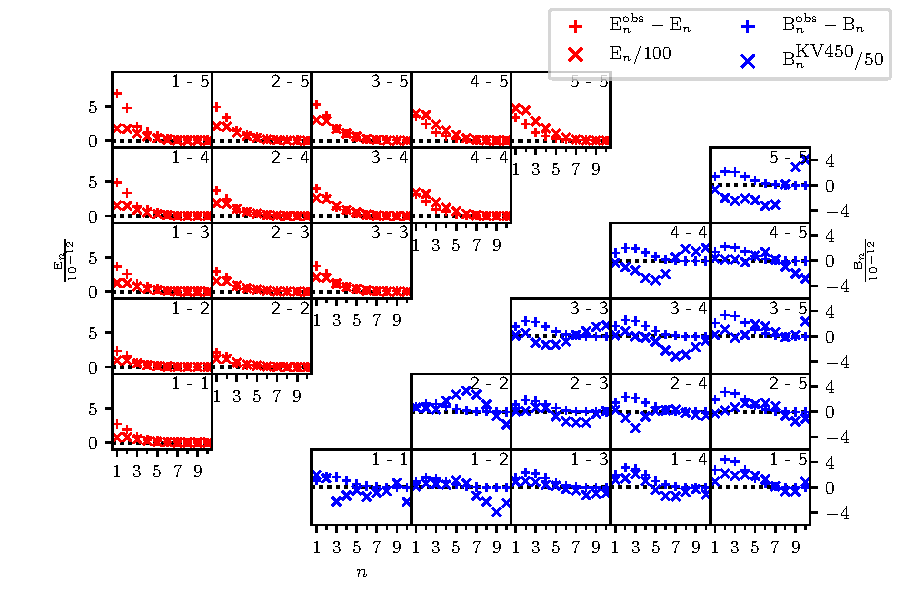
\includegraphics[width = \textwidth]{images/ebmodes0p5t72.pdf}
\caption{Difference in the E-modes (top left) and B-modes (bottom right) between the reference and the observed correlation functions. For comparison: Total E-modes of the reference correlation function $E_n$ (top left) and B-modes measured in the KV450 survey by Asgari et al. $B_n^{\rm{KV450}}$ (bottom right). All E- and B-modes were calculated using the logarithmic COSEBIS in S10 for an angular range of $\theta_{\rm{min}}=0.\!^\prime 5,\,\theta_{\rm{max}}=72\arcmin$.}
\label{fig:bmodes_cosebi}
\end{figure}

%-------------------------------------------------------------------

\section{Discussion}
\label{sec:discussion}
With our semi-analytic model we describe the impacts of varying depth in ground-based cosmic shear surveys. During our analysis we have made several simplifications, which we discuss below.
\begin{enumerate}
\item In the most general terms, we are analysing the effects of a position-dependent selection function on cosmic shear surveys. In our analysis, this selection function was governed by the KiDS $r$-band depth of a pointing. This neglects a number of other effects: The depth in different bands and the seeing of a pointing will also modify the number densities and redshift distributions on the scale of a pointing, whereas dithering strategies as well as imperfections in the telescope and CCD cause modifications on sub-pointing scales. However, we believe that these effects are subdominant compared to the variations caused by the $r$-band depth.

\item We have assumed an infinitely large survey area with an uncorrelated distribution of the depth-function. While the boundary effects arising from a finite survey footprint would have a small impact on the shape of the function $E(\theta)$\footnote{This would be due to the fact that a pointing next to a boundary has less neighbours, therefore making it more likely that a galaxy pair is in the same pointing.}, the governing factor is the sample variance of the depth-distribution. We have assumed that the probability that any pointing is of percentile $n$ is exactly the expectation value, namely $1/10$. While this is true for an infinitely large survey with an uncorrelated distribution of the depth-function, it does not necessarily hold for a real survey. However, our analysis in App.~\ref{sec:expand_eoftheta} suggests that these effects are not significant for the KV450 survey. In the models, we have also assumed an uncorrelated distribution of the depth-function. As can be seen in Fig \ref{fig:all_xis}, this approximation introduces a small error when compared to the simulations.

\item In our MCMC simulations we did not account for degeneracies with other cosmological parameters or observational effects. Especially intrinsic alignments and baryon feedback also modify the correlation functions primarily on small scales, so they are likely to be degenerate with the effect of varying depth \citep{Troxel:2015}. In an actual MCMC simulation that accounts for these effects, we suspect that the parameters for intrinsic alignments and baryonic feedback change to mitigate this effect, so that the impact on cosmological parameters is actually smaller than in our results. Also, possible degeneracies between $S_8$ and other cosmological parameters might bias the resulting values. %Furthermore, when including the effects of dark energy we notice that our observation of $S_8$ being constant is no longer valid: For a `Euclid-like' survey we notice a bias of $\sim 0.8\sigma$. This gives rise to the assumption that the results of an MCMC with the full parameter space, including observational effects, will differ from our results. 
\end{enumerate}

Despite these repercussions, we are confident to say that the effects of varying depth are not significant for the KV450 survey. The cosmological parameters did not change and the main parameter, $S_8$, is especially robust against this effect. In particular this means that a varying depth can not explain the discrepancy between observations of the local Universe and results from analysis of the CMB.

We have shown that this effect can create B-modes. However, \todo{cite new asgari et al. here as soon as it is on arxiv}\citet{2018arXiv181002353A} measured the B-modes of the KV450 survey in the same $\theta$-range. Those B-modes are greater than the ones created by varying depth by a factor of approx.~$50$ and show a completely different pattern, so it is safe to say that the B-modes in the KV450 survey are not created by varying depth. An interesting observation is that the change in E-modes is as big as the created B-modes (compare Fig.~\ref{fig:bmodes_cosebi}). This means that as soon as this effect causes a significant bias in the cosmological parameters, it will also create significant B-modes\footnote{While this is no big surprise, it is not trivial. It could be possible that a systematic effect only creates E-modes and no B-modes, which would be extremely unfortunate as it could bias cosmological parameters without ever being detected by a B-mode analysis.}. Additionally, the created pattern is very characteristic, which makes it easy to recognize in a B-mode analysis of an actual survey.

For next-generation surveys like Euclid, this effect will be significant. Although Euclid is a space-based telescope, the photometric redshift determination will still be done by ground-based telescopes and therefore suffer from the same effects. While we did not yet perform a quantitative study of this effect for Euclid, we are certain that a such a study should be conducted.

While the cosmology dependency (compare Fig. \ref{fig:comparecosmo}) is not significant for the KV450 survey, it will be relevant for the Euclid survey. In that case, a calculation of the correction for this effect is necessary for various cosmologies, underlining the necessity for a fast, analytic model. \todo{For that example I took value from the 95\% CL of KV450 from H18. As the parameter constraints in Euclid are going to be much tighter, this is probably no longer true...}

%As an outlook it would be interesting to perform a full MCMC simulation, including both cosmological and nuisance parameters. One might also check the most popular extensions to the standard model of cosmology, and see whether varying depth could cause a bias towards one of these models. Furthermore, the method developed in Appendix \ref{sec:expand_eoftheta} could be applied to the actual footprint of the KV450 survey to see whether finite field effects or a correlated distribution of $r$-band depth are significant.
Additionally, it is interesting to note that $E(\theta)$ is the azimuthal average of the function $E(\b\theta)$ derived in Sec.~\ref{sec:model_e}, which is not isotropic. Therefore, it would be possible to observe a direction-dependent correlation function $\xi_\pm^{ij,\rm{obs}}(\b\theta)$ in future surveys. An anisotropy in the observed correlation function could be a sign for the influence of varying depth.
\todo{Should we give an outlook? I.e. calculate covariances (I am trying to come up with something for that), apply to real KV450 footprint, ...}

%--------------------------------------------------------------------


\begin{acknowledgements}
We want to thank Jan-Luca van den Busch for his permission to use and modify his code for an MCMC simulation.\end{acknowledgements}


\bibliographystyle{aa}
\bibliography{cite}
\begin{appendix}
\section{Detailed Calculations}
\subsection{Calculation of the power spectrum}
In this Section we will perform the calculation for the observed power spectrum $P^{\text{obs}}(\b \ell)$. For this, we assume an infinitely large field in order to perform our integration over $\mathbb{R}^2$. In reality, finite field effects would play a role here. We begin with the calculation of the correlation for the Fourier transformed shear:
\begin{align}
& \la \gammaoh(\b \ell) \gammaoh {}^*(\b \ell')\ra\nonumber\\
 &\qquad = \la\int\text{d}^2 \theta\int\text{d}^2 \theta'\,W(\b \theta)W(\b \theta')\gamma(\b \theta)\gamma^*(\b \theta')\exp(\i \b \ell\b \theta-\i \b \ell'\b \theta')\ra\nonumber\\
 &\qquad = \la\int\text{d}^2 \theta\int\text{d}^2 \theta'\,W(\b \theta)W(\b \theta')\exp(\i \b \ell\b \theta-\i \b \ell'\b \theta') \int \frac{\text{d}^2 k}{(2\pi)^2}\int \frac{\text{d}^2 \ell}{(2\pi)^2}\, \hat{\gamma}(\b k)\hat{\gamma}^*(\b \ell)\exp(-\i \b k\b \theta+\i \b \ell\b \theta')\ra \nonumber\\
&\qquad = \la \int \text{d}^2 \theta \int \text{d}^2 \theta' \int \frac{\text{d}^2 k}{(2\pi)^2} \int \frac{\text{d}^2 \ell}{(2\pi)^2}\, P(\b k)(2\pi)^2 \delta(\b k-\b \ell) \exp[\i (\b \ell\b \theta-\b \ell'\b \theta'-\b k\b \theta+\b \ell\b \theta')]W(\b \theta)W(\b \theta')\ra \nonumber\\
  &\qquad = \la \int \frac{\text{d}^2 k}{(2\pi)^2} \, P(\b k) \int \text{d}^2 \theta\, W(\b \theta)\exp[\i\b \theta(\b \ell-\b k)]\int \text{d}^2 \theta'\, W(\b \theta') \exp[-\i\b \theta(\b \ell'-\b k)] \ra \nonumber\\
  &\qquad = \la \int\frac{\text{d}^2 k}{(2\pi)^2} \, P(\b k)\widehat{W}(\b \ell-\b k)\widehat{W}^* (\b \ell'-\b k)\ra
\end{align}
It is important to keep in mind that the ensemble averages of the weight function are independent of the ensemble averages of the shear values, meaning $\la W(\b \theta)\gamma(\b \theta)\ra = \la W(\b \theta)\ra \la \gamma(\b \theta)\ra$. We can define $W(\b \theta)=1+w(\b\theta)$ with $\la w(\b \theta)\ra = 0$, which leads to the expession
\begin{align}
& \la \gammaoh(\b \ell) \gammaoh {}^*(\b \ell')\ra \nonumber\\
 &\qquad = \la \int\frac{\text{d}^2 k}{(2\pi)^2} \, P(\b k) \left[ (2\pi)^4\delta(\b \ell-\b k)\delta(\b \ell'-\b k)+(2\pi)^2\big[ \hat{w}(\b \ell-\b k)\delta(\b \ell'-\b k) + \hat{w}^*(\b \ell'-\b k)\delta(\b \ell-\b k)\big]\right.\right. \nonumber\\
 & \quad\qquad \left.\left. + \hat{w}(\b \ell-\b k)\hat{w}(\b \ell'-\b k) \right] \right. \bigg> \nonumber\\
 &\qquad =  (2\pi)^2\delta(\b \ell-\b \ell')P(\b \ell) + \left[ \la \hat{w}(\b \ell-\b \ell')\ra P(\b \ell')+\la \hat{w}^*(\b \ell'-\b \ell)\ra P(\b \ell)\right] + \la \int \frac{\text{d}^2 k}{(2\pi)^2} \, \hat{w}(\b \ell-\b k)\hat{w}^*(\b \ell'-\b k)P(\b k)\ra \nonumber\\
& \qquad \overset{(*)}{=}  (2\pi)^2\delta(\b \ell-\b \ell')P(\b \ell) + \la \int \frac{\text{d}^2 k}{(2\pi)^2}\, \hat{w}(\b \ell-\b k)\hat{w}^*(\b \ell'-\b k)P(\b k)\ra \, ,
\label{eq:pobs1}
\end{align}
where in $(*)$ we have used that the average $\la \hat{w}(\b \ell)\ra$ vanishes.
Up until now, we have not specified our weight-function $w$. We parametrize it as \begin{equation}
w(\b \theta) = \sum_{\b \alpha \in \mathbb{Z}^2} w_{\b \alpha} \Xi(\b \theta-L\b \alpha)\text{ , with the Box-Function } \Xi(\b \theta) = \begin{cases}
1 \qquad \b \theta\in \left[-\frac{L}{2},\frac{L}{2}\right]^2 \\
0 \qquad \text{else}
\end{cases}.
\end{equation}
Here, the $w_{\b \alpha}$ are random variables, drawn from the random distribution describing the survey depths. For the Fourier transform we compute: \begin{equation}
\hat{w}(\b \ell) = \sum_{\b \alpha \in \mathbb{Z}^2} w_{\b \alpha} \exp(-\i \b \ell L\b \alpha) \widehat{\Xi}(\b \ell)\, ,
\end{equation}
where
\begin{equation}
\widehat{\Xi}(\b\ell) = \frac{4\sin\left(\frac{L\ell_1}{2}\right)\sin\left(\frac{L\ell_2}{2}\right)}{\ell_1\ell_2}\, ,
\label{eq:sinc}
\end{equation}
is a 2-dimensional sinc function.
Assuming an uncorrelated weight-distribution $\left(\la w_{\b \alpha} w_{\b \beta}\ra = 0\text{ for }\b \alpha\neq\b \beta\right)$ and setting $\la w^2\ra \equiv \la w_{\b \alpha}^2\ra$ for each $\b \alpha$, we get
\begin{align}
&\la \int \frac{\text{d}^2 k}{(2\pi)^2}\, \hat{w}(\b \ell-\b k)\hat{w}^*(\b \ell'-\b k)P(\b k)\ra \nonumber\\
&\qquad = \la \int \frac{\text{d}^2 k}{(2\pi)^2} \sum_{\b \alpha,\b \beta}w_{\b \alpha}w_{\b \beta} \exp[-\i(\b \ell - \b k)L\b \alpha]\, \widehat{\Xi}(\b \ell - \b k) \exp[\i(\b \ell' - \b k)L\b \beta]\, \widehat{\Xi}^*(\b \ell' - \b k)P(\b k)\ra \nonumber\\
&\qquad = \int \frac{\text{d}^2 k}{(2\pi)^2} \sum_{\b \alpha} \la w^2\ra \exp[-\i(\b \ell - \b k)L\b \alpha + i(\b \ell' - \b k) L\b \alpha]\, \widehat{\Xi}(\b \ell - \b k)\widehat{\Xi}^*(\b \ell' - \b k)P(\b k) \, .
\end{align}
Using this result, we can obtain the observed power spectrum \begin{equation}
P^{\rm{obs}}(\b\ell) = \frac{1}{(2\pi)^2}\int\d^2\ell' \la \gammaoh(\b \ell) \gammaoh {}^*(\b \ell')\ra\, ,
\end{equation}
by performing the $\b \ell'$-integration in \eqref{eq:pobs1}:
\begin{align}
P^{\text{obs}}(\b \ell) = & P(\b \ell)+\int \frac{\text{d}^2\b \ell'}{(2\pi)^2} \int\frac{\text{d}^2\b k}{(2\pi)^2}\sum_{\b \alpha}\la w^2\ra \exp[-\i(\b \ell-\b k)L\b \alpha+\i(\b \ell'-\b k)L\b \alpha]\, \widehat{\Xi}(\b \ell-\b k)\widehat{\Xi}(\b \ell' - \b k) P(\b k) \nonumber\\
= & P(\b \ell)+ \int\frac{\text{d}^2\b k}{(2\pi)^2}\sum_{\b \alpha}\la w^2\ra \exp[-\i(\b \ell-\b k)L\b \alpha]\, \widehat{\Xi}(\b \ell - \b k)P(k) \int\frac{\text{d}^2\b \ell}{(2\pi)^2}\, \widehat{\Xi}^*(\b \ell'-\b k)\exp[\i(\b \ell'- \b k)L\b \alpha] \nonumber\\
 = & P(\b \ell) + \la w^2\ra \int\frac{\text{d}^2\b k}{(2\pi)^2}\, \widehat{\Xi}(\b \ell-\b k)P(\b k) \sum_{\b \alpha}\exp[-\i(\b \ell - \b k)L\b \alpha]\,\Xi(L\b \alpha) \nonumber\\
 = & P(\b \ell) + \la w^2\ra \int\frac{\text{d}^2\b k}{(2\pi)^2}\,\widehat{\Xi}(\b \ell-\b k)P(\b k)\, ,
\end{align}
which is a convolution of the power spectrum and the 2-dimensional sinc function \eqref{eq:sinc}.
\label{sec:calc of PS}

\subsection{The function $E(\theta)$}
\label{sec:model_e}
When computing the shear correlation between a pair of galaxies, it is of central importance whether those two galaxies lie in the same pointing or not. We want to model the probability that a pair of galaxies with separation $\b\theta$ lie in the same pointing by the function $E(\b\theta)$, which we will derive here:

{
\def\vec{\b}
\begin{figure}
    \centering
    \def\svgwidth{200pt}    
    \hspace*{1cm}
    \input{images/eoftheta_new.pdf_tex}  
    \hspace*{-2cm}
    \caption[Graphic how to obtain $E(\b\theta)$]{Graphic representation on how to obtain the function $E(\b\theta)$. For a separation vector $\b\theta$, the dashed square represents the area of galaxies that have their partner in the same pointing.}
    \label{fig:explain_etheta}
\end{figure}
}
Given one square field of length $L$ (in our case $L=60\arcmin$) and a separation vector $\b\theta$, without loss of generality we can assume $\theta_1,\theta_2\geq 0$. The dashed square in Fig.~\ref{fig:explain_etheta} represents all possible positions that the first galaxy can take, such that the second galaxy is still within the same pointing. The volume of this square equals \begin{equation}
V(|\b\theta|,\phi)  = \big[L-|\b\theta|\cos(\phi)\big]\,\big[L-|\b\theta|\sin(\phi)\big]\, ,
\end{equation} where $\phi$ represents the angle of the vector $\b\theta$. The function $E(\b\theta)$ then simply equals $V(|\b\theta|,\phi)/L^2$. To exclude negative Volumes (which could occur when $|\b\theta|>1$ holds), we need to add the Heaviside theta function $\mathcal{H}$:
\begin{equation}
E(\b\theta)  = \left[1-\frac{|\b\theta|}{L}\cos(\phi)\right]\,\left[1-\frac{|\b\theta|}{L}\sin(\phi)\right]\, \mathcal{H}\left[1-\frac{|\b\theta|}{L}\cos(\phi)\right]\,\mathcal{H}\left[1-\frac{|\b\theta|}{L}\sin(\phi)\right]\, .
\label{eq:eoftheta1}
\end{equation} 
As $E(\b\theta)$ is not isotropic, in order to obtain the function $E(\theta) = E(|\b\theta|)$, we need to calculate the azimuthal average of Eq.~\eqref{eq:eoftheta1} over all angles $\phi$. While the case $\theta_1,\theta_2\geq 0$ certainly does not hold for all angles $\phi$, we can omit the other cases by making use of the symmetry of the problem.
\begin{align}
E(\theta) = & \frac{4}{2\pi}\int_0^{\frac{\pi}{2}}\d\phi\, E(\b\theta) = \frac{2}{\pi}\begin{cases}
\int_0^{\frac{\pi}{2}} \d\phi\, \left[1-\frac{|\b\theta|}{L}\cos(\phi)\right]\,\left[1-\frac{|\b\theta|}{L}\sin(\phi)\right]\, ,  & |\b\theta|  \leq L \\[10pt]
\int_{\cos\inv(L/|\b\theta|)}^{\sin\inv(L/|\b\theta|)} \d\phi\, \left[1-\frac{|\b\theta|}{L}\cos(\phi)\right]\,\left[1-\frac{|\b\theta|}{L}\sin(\phi)\right] \, , \quad   & L \leq |\b\theta| \leq \sqrt{2}L \\[10pt]
0\, , &\sqrt{2}L \leq\theta
\end{cases} \nonumber\\[10pt]
 = & \begin{cases}
\frac{1}{L^2 \pi}\left[L^2\pi - (4L-\theta) \theta\right]\, ,  & \theta \leq L \\[10pt]
\frac{2}{\pi}\,\left[4\sqrt{\frac{\theta^2}{L^2}-1} -1 - \frac{\theta^2}{2L^2} - \cos\inv\left(\frac{L}{\theta}\right) + \sin\inv\left(\frac{L}{\theta}\right)\right]\, ,  & L  \leq \theta \leq \sqrt{2}L \\[10pt]
0\, ,  & \sqrt{2}L \leq \theta
\end{cases}\, .
\end{align}

\subsection{Calculation of the shear correlation functions}
\label{sec:calc of xipm}
Following H17, given a set of galaxies we calculate the shear correlation function $\xi_+^{ij}$ via \begin{equation}
\xi^{ij}_+(\theta) = \frac{\sum_{a,b}w_a^iw_b^j\epsilon_a^i\epsilon_b^{j*}\Delta(|\b\theta_a^i-\b\theta_b^i|)}{\sum_{a,b}w_a^iw_b^j\Delta(|\b\theta_a^i-\b\theta_b^i|)}\, .
\label{eq:xip_from_observations}
\end{equation}
Here, $w$ represents the lensing weight of the galaxy, whereas $\epsilon$ is its (complex) ellipticity and $\b \theta$ its position on the sky. We have defined the function $\Delta$ as \[
\Delta(|\b\theta_a^i-\b\theta_b^i|) = \begin{cases}
1, \,\, & |\b\theta_a^i-\b\theta_b^j| \in [\theta,\theta+{\rm d}\theta] \\
0, & \text{ else}
\end{cases}\, ,
\]
where we assume ${\rm d}\theta \ll \theta$. We define $\mathcal{N}$ as the number of pointings in the survey and $F_k^i$ as the set of galaxies in pointing $k$ and tomographic redshift bin $i$. The numerator in Eq.~\eqref{eq:xip_from_observations} then transforms to: \begin{align}
& \sum_{k,\ell=1}^\mathcal{N} \sum_{a\in F_k^i}\sum_{b\in F_{\ell}^j} w_a^iw_b^j\epsilon_a^i\epsilon_b^{j*} \Delta(|\b\theta_a^i-\b\theta_b^i|) \nonumber\\
 = & \sum_{k=1}^\mathcal{N}\sum_{a\in F_k^i}w_a^i \sum_{\ell=1}^\mathcal{N} \sum_{b\in F_{\ell}^j} w_b^j \Delta(|\b\theta_a^i-\b\theta_b^i|)\, \epsilon_a^i\epsilon_b^{j*} \nonumber\\
  = & \sum_{k=1}^\mathcal{N}\sum_{a\in F_k^i}w_a^i \left[\sum_{b\in F_{k}^j} w_b^j \Delta(|\b\theta_a^i-\b\theta_b^i|)\, \epsilon_a^i\epsilon_b^{j*} + \sum_{\ell\neq k} \sum_{b\in F_{\ell}^j} w_b^j \Delta(|\b\theta_a^i-\b\theta_b^i|)\, \epsilon_a^i\epsilon_b^{j*}\right] \, .
\end{align}
When we denote the probability that pointing $k$ is of percentile $m$ by $\mathcal{P}_m^k$ and assume that the product $\epsilon_a^i\epsilon_b^{j*}$ always equals its expectation value, we can set the numerator as \[
\sum_{k=1}^\mathcal{N}\sum_{a\in F_k^i}w_a^i \sum_m \mathcal{P}_m^k \left[\overbrace{\sum_{b\in F_{k}^j} w_b^j \Delta(|\b\theta_a^i-\b\theta_b^i|)}^{\rm{(\ref{eq:numerator1}.a)}}\,  \xi_{+,mm}^{ij}(\theta) + \overbrace{\sum_{\ell\neq k} \sum_{b\in F_{\ell}^j} w_b^j \Delta(|\b\theta_a^i-\b\theta_b^i|)}^{\rm{(\ref{eq:numerator1}.b)}} \sum_n \mathcal{P}_n^{\ell} \xi_{+,mn}^{ij}(\theta)\right] \, .
\label{eq:numerator1}
\]
The term (\ref{eq:numerator1}.a) denotes all galaxies that lie within distance interval $[\theta,\theta+{\rm d}\theta]$ of galaxy $a$, and are in the same pointing as galaxy $a$. This term is equal to the (weighted) number density of galaxies in the pointing multiplied by $2\pi\theta\, {\rm d}\theta\, E(\theta)$. 

The term (\ref{eq:numerator1}.b) denotes all galaxies within distance interval $[\theta,\theta+{\rm d}\theta]$ of galaxy $a$, that are \textit{not} in the same pointing as galaxy $a$. This is equal to the number density of galaxies in the respective pointings multiplied by $2\pi\theta\, {\rm d}\theta\, [1-E(\theta)]$. 
 
If we assume that said number density in a pointing is equal to the number density in the percentile it belongs to, $N_n^j$, and set $\mathcal{P}_n^\ell=1/10$, the numerator becomes \begin{align}
\sum_{k=1}^\mathcal{N} \sum_{a\in F_k^i} w_a^i \sum_m P^k_m \left[2\pi\theta\,\d\theta\,E(\theta) N_m^j \xi_{+,mm}^{ij}(\theta) + 2\pi\theta\,\d\theta\,\frac{1-E(\theta)}{10}\, \sum_n N_n^j \xi_{+,mn}^{ij}(\theta) \right] \, .
\end{align}
The term $\sum_{a\in F_k^i} w_a^i$ denotes the number of galaxies in pointing $k$, which we set as the number density of galaxies in the respective percentile multiplied with the area $A$ of the pointing. Applying this and setting $\mathcal{P}_m^k=1/10$, the numerator reads 
\begin{align}
\frac{2\pi\theta\,\d\theta}{10} \sum_{k=1}^\mathcal{N} \sum_m N_m^i A &\left[ E(\theta) N_m^j \xi_{+,mm}^{ij}(\theta) + \frac{1-E(\theta)}{10}\sum_n N_n^j\xi_{+,mn}^{ij}(\theta)\right] \nonumber\\
 =  \, \frac{2\pi\theta\,\d\theta \, NA}{10}  \sum_m N_m^i &\left[ E(\theta) N_m^j \xi_{+,mm}^{ij}(\theta) + \frac{1-E(\theta)}{10}\sum_n N_n^j\xi_{+,mn}^{ij}(\theta)\right] \, .
\end{align}
%
 The same line of argumentation can be applied to the denominator, which then reads: \[
\frac{2\pi\theta\,\d\theta \, NA}{10}  \sum_m N_m^i \left[ E(\theta) N_m^j + \frac{1-E(\theta)}{10}\sum_n N_n^j\right]\, .
 \]
Taking the ratio of the two quantities, we see that Equations \eqref{eq:xip_from_observations} and \eqref{eq:correctionfunction1} are the same\footnote{Note that while here $N_m^i$ denotes a number density, in Equations \eqref{eq:xip_from_observations} and \eqref{eq:correctionfunction1} it denotes the total (weighted) number of galaxies. However, the difference is just a multiplication with the area $A$ of the pointings, which appears both in the numerator and the denominator and is thus cancelled out.}.
\section{Finite field effects}
\label{sec:expand_eoftheta}
\begin{figure}
    \centering
    \def\svgwidth{200pt}    
%    \hspace*{1cm}
    \input{images/expand_eoftheta.pdf_tex}  
%    \hspace*{-2cm}
    \caption{Graphic representation of the definitions of $E_{ab}(\theta)$. When the first galaxy is in the bottom left pointing, the probability to find the second galaxy in a pointing of distance $(a,b)$ is $E_{ab}(\theta)$.}
    \label{fig:expand_etheta}
\end{figure}
In this chapter we will outline how to calculate the correction of the correlation functions for a finite survey with a potentially correlated distribution of depth between pointings. Essentially, this boils down to the calculation of $\mathcal{P}_{mn}^{ij}(\theta)$ from Equation \eqref{eq:def_xiobs}. We calculate this weighting by the geometrical probability that a pair of galaxies of separation $\theta$ is of percentiles $m$ and $n$, $\mathcal{P}(m,n|\theta)$, weighted by the respective number of galaxies in the percentiles $N_m^i,N_n^j$: \[
\mathcal{P}_{mn}^{ij}(\theta) = N_m^iN_n^j\mathcal{P}(m,n|\theta)\, .
\label{eq:pmnij1}
\]
 At first we define Functions $E_{ab}(\b\theta)$ as the probabilty that a galaxy pair of separation $\b\theta$ is in pointings of distance $(a,b)$. This situation is depicted in Fig.~\ref{fig:expand_etheta}. Due to symmetry, for the azimuthal average of the functions, $E_{ab}(\theta) = E_{-ab}(\theta) = E_{ba}(\theta)$ holds for all combinations of $a$ and $b$. Note that $E_{00}(\theta)=E(\theta)$ and $\sum_{a,b}E_{ab}(\theta)\equiv 1$.

Let $\mathcal{P}^*(m,n|a,b)$ denote the probability that two pointings of distance $(a,b)$ are of percentile $m$ and $n$ (which is directly calculable from a given survey footprint). 
Then the following equation holds: \[
\mathcal{P}(m,n|\theta) = \sum_{a,b} E_{ab}(\theta)\mathcal{P}^*(m,n|a,b)\, .
\label{eq:pmntheta}
\]
Note that the expectation value of $\mathcal{P}^*(m,n|a,b)$ for uncorrelated distributions is \[
\la \mathcal{P}^*(m,n|a,b)\ra = \begin{cases}
0.1\,\delta_{mn},\qquad & \text{for }(a,b)=(0,0) \\
0.01, & \text{else}
\end{cases}\, ,
\label{eq:pmnabstar}
\]
where $\delta_{mn}$ denotes the Kronecker delta. Keeping in mind that \[
\sum_{(a,b)\neq (0,0)} E_{ab}(\theta) = 1-E(\theta)\, ,
\]
we can use the expectation value \eqref{eq:pmnabstar} to calculate \eqref{eq:pmntheta} as a consistency check. In that case, we receive the same value for the coefficients in \eqref{eq:pmnij1} as we have in Eq. \eqref{eq:pmnij_uncorr} in Sec. \ref{sec:xipm_semianalytic} for the case of an infinite footprint and uncorrelated distribution of depth.

\begin{figure}
\centering
\begin{subfigure}[c]{0.49\textwidth}
\def\svgwidth{100pt}
\hspace*{2cm}
\input{images/e_1.pdf_tex}
\subcaption{For $\theta\sin(\phi)<L$ the volume of the dashed rectangle is $V(\theta,\phi)=\theta\sin(\phi)[L-\theta\cos(\phi)]$.}
\label{fig:e01thetaa}
\end{subfigure}
\begin{subfigure}[c]{0.49\textwidth}
\def\svgwidth{100pt}
\hspace*{2cm}
\input{images/e_2.pdf_tex}
\subcaption{For $\theta\sin(\phi)>L$ the volume of the dashed rectangle is $V(\theta,\phi)=[2L-\theta\sin(\phi)]\, [L-\theta\cos(\phi)]$.}
\label{fig:e01thetab}
\end{subfigure}
\caption[How to calculate $E_{01}(\theta)$]{How to calculate $E_{01}(\theta)$ for different values of $\theta$.}
\label{fig:e01theta}
\end{figure}

The $E_{ab}$ can all be calculated analytically, similar to our method in Sec. \ref{sec:model_e}. We again assume a selection of square fields with side length $L$, and later set $L=60\arcmin$ to adapt to the KV450 survey. As an example, for $E_{01}$ we have several possible situations, depicted in Fig. \ref{fig:e01theta}. Setting $E_{ab}(\b\theta) = V(\theta,\phi)/L^2$, we define \begin{align}
E_{01}^{(a)}(\b\theta) & \equiv \frac{\theta}{L}\sin(\phi)[1-\frac{\theta}{L}\cos(\phi)] \nonumber\\
E_{01}^{(b)}(\b\theta) & \equiv [2-\frac{\theta}{L}\sin(\phi)]\, [1-\frac{\theta}{L}\cos(\phi)]
\end{align}
With some geometric considerations, we compute:
{
\begingroup
\addtolength{\jot}{1em}
\begin{align}
E_{01}(\theta) = & \begin{cases}
\frac{1}{\pi}\int_0^{\frac{\pi}{2}} \d\phi\, E_{01}^{(a)}(\b\theta), & \frac{\theta}{L} < 1 \\[10pt]
 \frac{1}{\pi}  \left[\int_{\cos\inv(L/\theta)}^{\sin\inv(L/\theta)}\d\phi\,E_{01}^{(a)}(\b\theta) + \int_{\sin\inv(L/\theta)}^{\frac{\pi}{2}}\d\phi\, E_{01}^{(b)}(\b\theta) \right],  & 1 < \frac{\theta}{L} < \sqrt{2} \\[10pt]
 \frac{1}{\pi} \int_{\cos\inv(L/\theta)}^{\frac{\pi}{2}}\d\phi\, E_{01}^{(b)}(\b\theta), & \sqrt{2}<\frac{\theta}{L}<2 \\[10pt]
\frac{1}{\pi} \int_{\cos\inv(L/\theta)}^{\sin\inv(2L/\theta)}\d\phi\, E_{01}^{(b)}(\b\theta), & 2<\frac{\theta}{L}<\sqrt{5} \\[10pt]
 0, & \sqrt{5}<\frac{\theta}{L}
\end{cases}\nonumber\\
 = & \begin{cases}
 \frac{(2L-\theta)\theta}{2\pi L^2}, & \frac{\theta}{L} < 1 \\[10pt]
 \frac{1}{\pi}\left[\frac{3}{2}- 2\frac{\theta}{L}+\frac{\theta^2}{L^2}+2\sqrt{\frac{\theta^2}{L^2}-1}+2\rm{sec\inv}\left(\frac{\theta}{L}\right)\right], & 1<\frac{\theta}{L}<\sqrt{2} \\[10pt]
 \frac{1}{2\pi}\left[-1-4\frac{\theta}{L}+4\sqrt{\frac{\theta^2}{L^2}-1}+4\rm{csc\inv}\left(\frac{\theta}{L}\right)\right], & \sqrt{2} < \frac{\theta}{L} < 2 \\[10pt]
 \frac{1}{2\pi}\left[-5-\frac{\theta^2}{L^2}+2\sqrt{\frac{\theta^2}{L^2}-4}+4\sqrt{\frac{\theta^2}{L^2}-1}-4\rm{sec\inv}\left(\frac{\theta}{L}\right)+4\sin\inv\left(\frac{2L}{\theta}\right)\right], & 2 < \frac{\theta}{L} < \sqrt{5} \\[10pt]
 0, & \sqrt{5}<\frac{\theta}{L}
 \end{cases}\, .
\end{align}
\endgroup
}

\begin{figure}
\centering
\def\svgwidth{120pt}
\input{images/drawing.pdf_tex}
\caption[Visualisation of the numerical computation for $E_{01}(\theta)$.]{Visualisation of the numerical computation for $E_{01}(\theta)$. For a circle of radius $\theta$, the length of the red arc divided by $2\pi$ represents the fraction of galaxies within the respective pointing. This value needs to be integrated for all possible centers of the circle in the pointing. That procedure is straightforward to expand for other $E_{ab}(\theta)$.}
\label{fig:eoftheta_sim}
\end{figure}

\begin{figure}
\centering
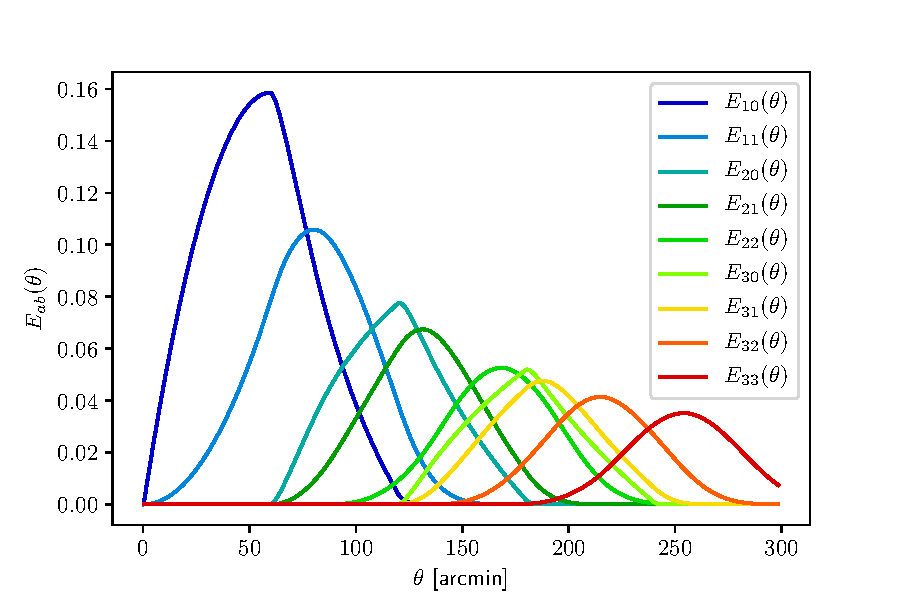
\includegraphics[width = 0.8\textwidth]{images/eab.pdf}
\caption{The functions $E_{ab}(\theta)$ for the first few possible combinations.}
\label{fig:eab}
\end{figure}
Naturally, to calculate those functions for all possible combinations would be rather tedious, however they are simple to determine numerically (compare Fig.~\ref{fig:eoftheta_sim}). A plot of these functions can be found in Fig.~\ref{fig:eab}.

\begin{figure}
\centering
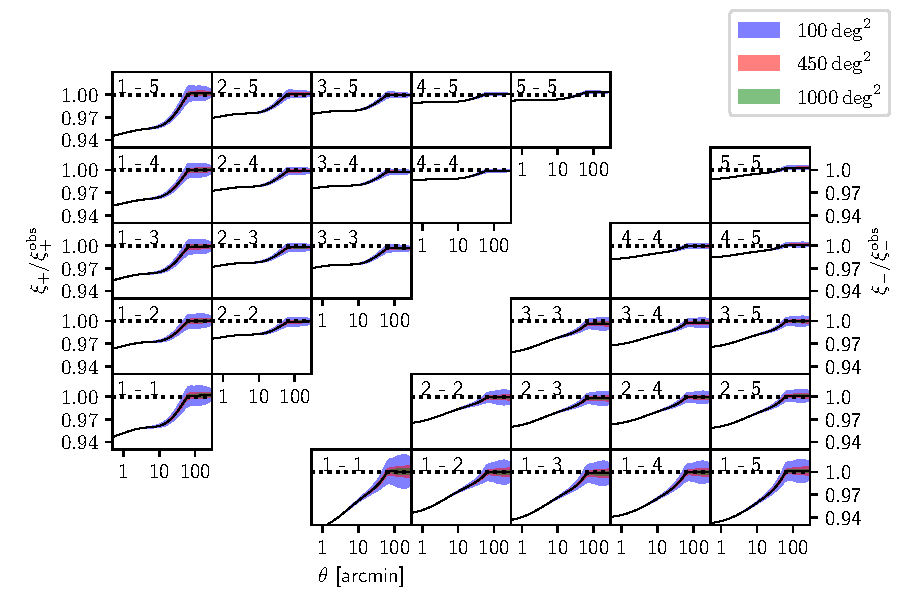
\includegraphics[width=\textwidth]{images/finite_footprint.pdf}
\caption{$2\sigma$-contours of the corrections for the correlation functions for a $100\,\rm{deg}^2$ field (blue), a $450\,\rm{deg}^2$ field (red) and a $1000\,\rm{deg}^2$ field (green).}
\label{fig:finite_footprint}
\end{figure}

We sampled several realizations of a random depth-distribution for a $100\,\rm{deg}^2$-field, a $450\,\rm{deg}^2$-field and a $1000\,\rm{deg}^2$-field and computed the variance of the resulting correlation functions. As can be seen from Fig. \ref{fig:finite_footprint}, the effect is quite significant for a $100\,\rm{deg}^2$-field, but almost negligible for a $1000\,\rm{deg}^2$-field. This leads to the assumption that both for the KV450 survey as well as for all next-generation cosmic shear surveys, finite field effects do not need to be accounted for. However, if the distribution of depth is correlated in the surveys, that might have a noticeable impact on the results.

\section{Additional Figures}

\begin{figure}[h]
\centering
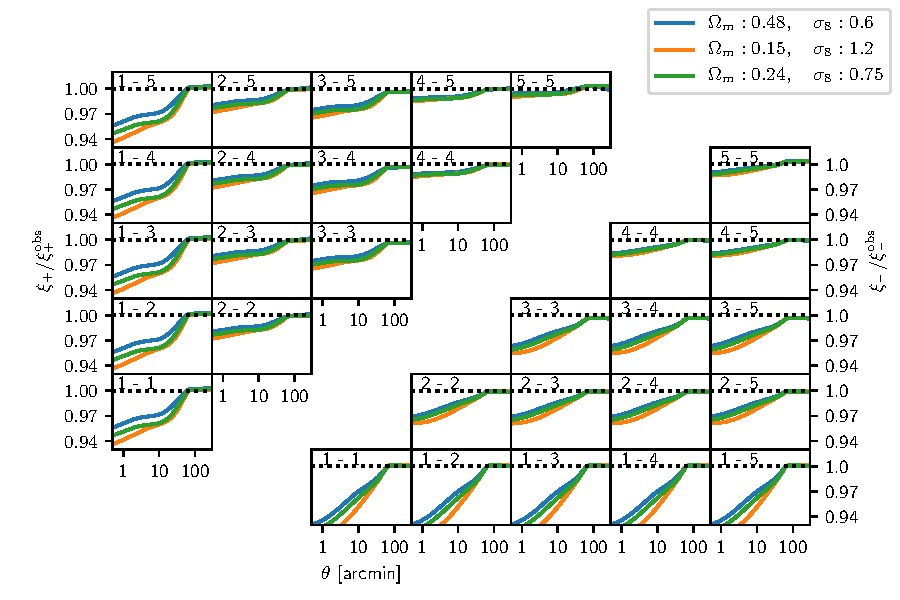
\includegraphics[width=\textwidth]{images/compare_cosmos.pdf}
\caption{Correction to the correlation functions in varying cosmologies. Depicted here are three flat sample cosmologies, where values within the 98\% CL of the KV450 survey were sampled.}
\label{fig:comparecosmo}
\end{figure}
\end{appendix}
\end{document}
%
